%\documentclass[notes=onlyslideswithnotes]{beamer}
\documentclass[notes=hide]{beamer}
%\documentclass[notes]{beamer}
%\documentclass[11pt,letterpaper]{article}
%\usepackage{beamerarticle}

\usepackage{genchem}
\usepackage{lecture}
\usepackage{multicol}
\usepackage{modiagram}
\usepackage{elements}
%\usepackage{ccicons}

\renewcommand*\printangularmomentum[1]{#1}

\usepackage{orbitalfilling}[2019/02/14]

\title{Periodic Properties of the Elements}
\subtitle{Chapter 3}
\institute[CHEM115 Bloomsburg University]{CHEM115 --- Chemistry for the Sciences I \\ Bloomsburg University}
\author{CHEM115 - Chemistry for the Sciences I}
\date{Spring 2019}

\begin{document}

\begin{frame}{Atomic Radii}
	How does the effective nuclear charge affect other atomic properties?

	\begin{center}
		\includegraphics[scale=0.4,trim={0 0 0 40pt},clip]{atomic-radii.jpg}
	\end{center}
\end{frame}

\begin{frame}{Ionic Radii}
	\centering
	\includegraphics[scale=0.4]{cationic-radii.jpg}
	\qquad
	\includegraphics[scale=0.4]{anionic-radii.jpg}
\end{frame}

\begin{frame}{Comparing Relative Radii}
	Rank the following ions in order of decreasing ionic radii by
	filling in the table below:
	
	\begin{center}
		\ch{Na+} \hspace{2em} \ch{Mg^{2+}} \hspace{2em} \ch{Al^{3+}}
	\end{center}

	\begin{center}
		\begin{tabu} to \linewidth {>{\bfseries}X[l] X[c] X[c] X[c]}
			\toprule\rowfont{\bfseries} & \ch{Na+} & \ch{Mg^{2+}} & \ch{Al^{3+}} \\
			\midrule
			\ch{e-} config \\[1em]
			\# protons \\[1em]
			\# electrons \\[1em]
			$\bm{Z_\text{eff}}$ \\[1em]
			\bottomrule
		\end{tabu}
	\end{center}

	\note{
		\begin{tabu} spread 1em {>{\bfseries}X[l] X[c] X[c] X[c]}
			\toprule\rowfont{\bfseries} & \ch{Na+} & \ch{Mg^{2+}} & \ch{Al^{3+}} \\
			\midrule
			\ch{e-} config & \elconf{Ne} & \elconf{Ne} & \elconf{Ne} \\
			\# protons & 11 & 12 & 13 \\
			\# electrons & 10 & 10 & 10 \\
			$\bm{Z_\text{eff}}$ & +1 & +2 & +3 \\
			\bottomrule
		\end{tabu}}
\end{frame}

\begin{frame}{Some notes on forming ions\ldots}
	\begin{itemize}[<+->]
		\item For \emph{main group elements}, electrons are removed in
			the reverse order of filling.

			\begin{center}
				\begin{tabu} spread 1em {X[-1,l] X[-1,c] X[-1,l]}
					F = \elconf{F} & $\rightarrow$ & \ch{F-} =
					$1s^22s^22p^{\color{red}6}$ \\
					Li = \elconf{Li} & $\rightarrow$ &
					\ch{Li+} = $1s^22s^{\color{red}0}$ or
					\elconf{He} \\
				\end{tabu}
			\end{center}

		\item For \emph{transition elements}, remove the electrons in
			the highest $n$-value orbitals first, even if this does
			not correspond to the reverse order of filling.

			\begin{center}
				\begin{tabu} spread 1em {X[-1,l] X[-1,c] X[-1,l]}
					V = [Ar]$4s^23d^3$ & $\rightarrow$ &
					\ch{V^{2+}} =
					[Ar]$4s^{\color{red}0}3d^3$ or
					[Ar]$3d^3$
				\end{tabu}
			\end{center}

			This deviation has been confirmed experimentally -- in
			particular, this agrees well with the \emph{magnetic
			properties} of the elements/ions.
	\end{itemize}
\end{frame}

\begin{frame}{The Magnetic Properties of Ions}
	Recall $m_s$ -- What does it mean to have a spin of $\pm\frac{1}{2}$?

	\pause

	\begin{description}
		\item[Paramagnetic:] The atom or ion is \emph{attracted} to a
			magnetic field.
	\end{description}

	\begin{center}
		\begin{tabu} spread 1em {*{2}{X[-1,l]} *{2}{X[-1,c]}}
			\ch{Ag} & [\ch{Kr}]$5s^14d^{10}$ &
			\electronup & \electronboth \electronboth
			\electronboth \electronboth \electronboth \\
			& & $5s$ & $4d$
		\end{tabu}
	\end{center}

	\begin{description}
		\item[Diamagnetic:] The atom or ion is \emph{slightly repelled}
			by a magnetic field.
	\end{description}

	\begin{center}
		\begin{tabu} spread 1em {*{2}{X[-1,l]} *{2}{X[-1,c]}}
			\ch{Zn} & [\ch{Ar}]$4s^23d^{10}$ &
			\electronboth & \electronboth \electronboth
			\electronboth \electronboth \electronboth \\
			& & $4s$ & $3d$ \\
			\ch{Zn^{2+}} & [\ch{Ar}]$4s^03d^{10}$ &
			\electronnone & \electronboth \electronboth
			\electronboth \electronboth \electronboth \\
			& & $4s$ & $3d$
		\end{tabu}
	\end{center}
\end{frame}

\begin{frame}{Identifying Magnetism}
	Write the electron configuration and orbital diagram for each ion and
	determine whether each is diamagnetic or paramagnetic.

	\tabulinesep=2em
	\begin{tabu} spread 1em {X[-1,l] *{2}{X[c]}}
		\ch{Al^{3+}}  \\
		\ch{Fe^{3+}}  \\
		\ch{Fe^{2+}}  \\
	\end{tabu}

	\note{
	\tabulinesep=2em
	\begin{tabu} spread 1em {X[-1,l] *{2}{X[c]}}
		\ch{Al^{3+}} & \elconf{Ne} & diamagnetic \\
		\ch{Fe^{3+}} & [Ar]$3d^5$ & paramagnetic \\
		\ch{Fe^{2+}} & [Ar]$3d^6$ & paramagnetic \\
	\end{tabu}}
\end{frame}

\begin{frame}{How easy is it to remove an electron?}
	\begin{columns}
		\column{0.45\linewidth}
		\begin{itemize}[<+->]
			\item We have calculated the energies of atomic orbitals
				before:
				\begin{equation*}
					E_n = R_{\ch{H}} \bigg( \frac{Z^2}{n^2} \bigg)
				\end{equation*}
			\item As we increase in $n$, we noted that the energy of
				the orbital \emph{increased}.
			\item What happens if we keep increasing $n$?
		\end{itemize}
		\column{0.45\linewidth}
		\visible<3->{
		\begin{center}
			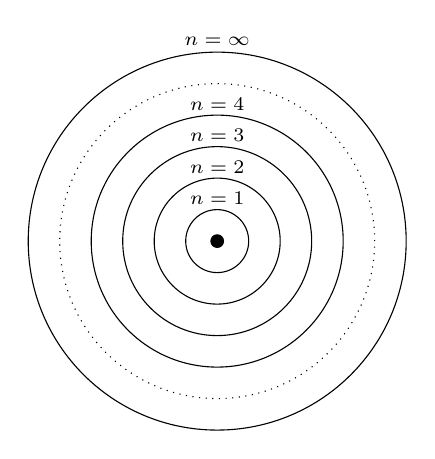
\begin{tikzpicture}[scale=0.4]
				\tikzstyle{every node} = [font=\scriptsize];
				\filldraw[black] (0,0) circle (0.2);
				\foreach \x in {1,2,...,4} {
					\draw[black] (0,0) circle (\x);
					\node[yshift=4pt] at (0,\x) {$n =
					\x$};
					}
				\draw[dotted,black] (0,0) circle (5);
				\draw[black] (0,0) circle (6);
				\node[yshift=4pt] at (0,6) {$n = \infty$};
			\end{tikzpicture}
		\end{center}}
	\end{columns}

	\visible<4->{
	\begin{block}{Ionization Energy}
		 The energy required to remove an electron from the atom or ion
		 in the gaseous state. Ionization energy is \emph{always}
		 positive because removing an electron always takes energy. 
	\end{block}}
\end{frame}

\begin{frame}[allowframebreaks]{First Ionization Energy}
	The energy required to remove the \emph{first} electron is the
	\emph{first ionization energy}.

	\begin{reaction*}
		Na\gas{} + \text{energy} -> Na^{+}\gas{} + 1 \el
	\end{reaction*}
		
	\begin{itemize}
		\item Decreases going down a group as the distance between the
			nucleus and valence electrons increases.
		\item Increases going across a period from left to right due to
			greater effective nuclear charge.
	\end{itemize}

	\framebreak

	\begin{center}
		\includegraphics[scale=0.4,trim={0 0 0
		40pt},clip]{first-ionization.jpg}
	\end{center}
\end{frame}

\begin{frame}[allowframebreaks]{Second (and Successive) Ionization Energy}
	\begin{columns}
		\column{0.35\linewidth}
		The energy required to remove an electron from an \emph{ion} is
		generally higher than the first ionization energy.
		
		\begin{reactions*}
			&Na^{+}\gas{} + \text{energy} \\
			&\qquad -> Na^{2+}\gas{} + 1 \el
		\end{reactions*}
		\column{0.55\linewidth}
		\begin{center}
			\includegraphics[scale=0.3]{successive-ionization.jpg}
		\end{center}
	\end{columns}

	\framebreak

	\begin{center}
		\includegraphics[scale=0.42]{ionization-energies.jpg}
	\end{center}
\end{frame}

\begin{frame}{What about gaining electrons?}
	\begin{block}{Electron Affinity}
		The energy change associated with gaining an electron in the
		gaseous state. \emph{Usually negative} because energy is
		released as electrons are gained.
	\end{block}

	\begin{reaction*}
		Cl\gas{} + 1 \el{} -> Cl^{-}\gas{} + \text{energy}
	\end{reaction*}

	\begin{columns}
		\column{0.45\linewidth}
		\begin{itemize}
			\item No significant trend down a column.
			\item Generally becomes more negative across a row.
		\end{itemize}
		\column{0.45\linewidth}
		\begin{center}
			\includegraphics[scale=0.2]{electron-affinities.jpg}
		\end{center}
	\end{columns}
\end{frame}

\begin{frame}{Trends in Metallic Character}
	\begin{center}
		\includegraphics[scale=0.42,trim={0 0 0
		40pt},clip]{metallic-character.jpg}
	\end{center}
\end{frame}

\begin{frame}
	\begin{center}
		\includegraphics[scale=0.42]{summary.jpg}
	\end{center}
\end{frame}

\end{document}
